\section{Message Board}
\Writetofile{hints}{\protect\section{Message Board 4}}
\Writetofile{soln}{\protect\newpage\protect\section{Message Board 4}}

\subsection{Problem 1}
\begin{enumerate}
    \item Given a point outside a circle, construct a line through the point tangent to the circle.


    \item Given two nonintersecting circles, construct all lines tangent to both.
    
    
    \item Given the lengths of two sides of a triangle and the length of the median to the third side, construct the triangle.
    
\end{enumerate}

\begin{mdsoln}
    Solution outline to 1:
Let $P$ be the point and $\omega$ the circle. Let $\omega$ have center $O$. Construct the circle $\omega_1$ with diameter $OP$. It must intersect $\omega$ in two points $A$ and $B$. Then, $PA\perp OA$, so $PA$ is tangent to $\omega$, as desired. ($PB$ is also tangent to $\omega$.)

Solution outline to 2:
Let $\omega_1$ and $\omega_2$ be the two circles, with centers $O_1$ and $O_2$, respectively. Construct the line perpendicular to $O_1O_2$ at $O_1$, and let this line meet $\omega_1$ at $A$ and $B$. Likewise, construct the line perpendicular to $O_1O_2$ at $O_2$, and let this line meet $\omega_2$ at $C$ and $D$, such that $A$ and $C$ are on the same side of line $O_1O_2$.

If $\omega_1$ and $\omega_2$ have the same radius, then it is evident that their common external tangents are given by $AC$ and $BD$. Otherwise, $AC$ and $BD$ are not parallel, so we may construct their intersection point $P$. Then, $P$ is the center of the homothety with positive ratio taking $\omega_1$ to $\omega_2$, since $A$ and $C$ are corresponding points on $\omega_1$ and $\omega_2$, as are $B$ and $D$. Hence, $P$ must be the intersection of the common external tangents of $\omega_1$ and $\omega_2$. Having found $P$, we can then use the method described to our solution to part 1 of this problem to construct both common external tangents to $\omega_1$ and $\omega_2$.

$AD$ and $BC$ cannot be parallel, so we can construct their intersection point $Q$. Then, $Q$ is the center of the homothety with negative ratio taking $\omega_1$ to $\omega_2$, since $A$ and $D$ are corresponding points on $\omega_1$ and $\omega_2$, as are $B$ and $C$. Hence, $Q$ must be the intersection of the common internal tangents of $\omega_1$ and $\omega_2$. Having found $Q$, we can again use our method of part 1 to construct both common internal tangents to $\omega_1$ and $\omega_2$, and we are done.

Solution outline to 3:
Let the desired triangle be $ABC$, with side lengths $a$ and $c$ and median $m_B$ (from $B$ to the midpoint of $CA$) given. Let $D,E,F$ be the midpoints of $BC,CA,AB$, respectively. Clearly, $DE = c/2$, $DB = a/2$, $BE = m_B$, so $c/2\le a/2 + m_B$, by the Triangle Inequality.

Construct $PQ$ of length $c$, and construct its midpoint $M$. Construct then a circle $\omega_1$ of radius $a/2$ and another of radius $m_B$ about $Q$. Since $MQ = c/2$, and since $c/2\le a/2 + m_B$, $\omega_1$ and $\omega_2$ must intersect in at least one point. Pick $N$ one such intersection point (the two choices of $N$ are equivalent up to reflection about line $PQ$). Then, construct $R$ on ray $PN$ with $PR = 2PN$.

Since $PR = 2PN$ and $PQ = 2PM$, we have $\triangle PMN\sim \triangle PQR$, so $QR = 2MN = a$. We conclude that $\triangle PQR$ is a triangle with $PQ = c$, $QR = a$, and the median from $Q$ of length $m_B$, and hence a solution to the problem.

It is simple to prove that this construction indeed constructs the only possible triangle satisfying the conditions of the problem.

\end{mdsoln}
\subsection{Problem 2}

Given the lengths of the three medians of a triangle, construct the triangle.

\textit{Has hints.}
\begin{sketch}
    Do this one first: Given the lengths of two sides of a triangle and the length of the median to the third side, construct the triangle.    
\end{sketch}

\begin{mdsoln} \ \\
    \begin{lemma}
        Given a segment $XY$, we can trisect it (that is, find $Z$ on $XY$ such that $YZ = XY/3$).
    \end{lemma}
    \begin{proof}
        Construct a circle of arbitrary radius about $Y$ and find a diameter $PQ$ of it with $P$ not collinear with $X$ and $Y$. Then, find the centroid $Z$ of triangle $XPQ$. Since $XY$ is a median of this triangle, $Z$ must lie on segment $XY$ with $YZ = XY/3$ - and so we are done.
    \end{proof}
 
\vspace{6pt}
Let $m_A$, $m_B$, and $m_C$ be the lengths of the three given medians.

Using the tactics of Problem 1, part 3, construct (the only possible) triangle $GAB$ with two side lengths $GA = 2m_A/3$ and $GB = 2m_B/3$, and the median from $G$ to $AB$ of length $m_C/3$. (Note that we can isolate these lengths because of the Lemma.)

Then, construct $D$ on ray $AG$ such that $AD = m_A$ and construct $E$ on ray $BG$ such that $BE = m_B$.

Now, by our construction we see that $GDE\sim GAB$ with ratio $1: 2$. Hence, $DE\parallel AB$ so $AE$ and $BD$ must intersect at some point $C$ which is the center of a homothety taking $DE$ to $BA$. Since $2DE = BA$, this homothety must have ratio 2. We conclude that $D$ is the midpoint of $BC$ and $E$ the midpoint of $CA$, so $G$ is the centroid of $\triangle ABC$. It is clear then that the lengths of the medians of $\triangle ABC$ from $A$ and $B$ are $m_A$ and $m_B$, respectively. The median from $C$ must be of length $3GM$ where $M$ is the midpoint of $AB$. But we know $GM = m_C/3$, so the median from $C$ in $\triangle ABC$ must have length $m_C$. Therefore, $\triangle ABC$ is a triangle of the desired form.

It is again simple to prove that our construction finds the only possible triangle satisfying the conditions of the problem.

\end{mdsoln}

\subsection{Problem 3}

In class we did this problem:

Construct a triangle $ABC$ given the feet of the altitudes from $D$, $E$, and $F$ (assume points $D$, $E$, and $F$ are distinct).

Prove that our construction does in fact produce a triangle $ABC$ with the desired property.

Also, is this $ABC$ unique? (That is, are there other possible triangles $ABC$ with the property that the given $DEF$ is the orthic triangle of $ABC$.)

\begin{mdsoln}
    Suppose that our construction produces triangle $ABC$ and that $DEF$ has incenter $H$. Then, by our construction, we have $\angle HEA = 180^\circ - \angle AFH = 90^\circ$, so $AEHF$ is cyclic, implying that $\angle CAB = \angle EAF = 180^\circ - \angle FHE$. It is fairly simple to prove that since $H$ is the incenter of $DEF$, $\angle FHE = 90^\circ + \angle FDE/2$. Then,
    \begin{align*}\angle CAB & =  180^\circ - \angle FHE \\
    & =  90^\circ - \angle FDE/2 \\
    & = 90^\circ - \angle ADE \\
    & =  90^\circ - \angle HCE\end{align*}where the last step follows since $CDHE$ is cyclic. Then, $\angle CAB = 90^\circ - \angle FCA$, so $F$ is the foot of the altitude from $C$ to $AB$. Likewise, $AD$ and $BE$ must also be altitudes of $ABC$, as desired.
    
    In general, the triangle $ABC$ is not unique. For example, note that the orthic triangle of triangle $ABH$ is also triangle $DEF$.
    \begin{center}
    \begin{asy}
        import cse5;
        import olympiad;
 

    size(150);
    pathpen = black + linewidth(0.7);
    pointpen = black;
    pen s = fontsize(8);
    
    pair A = dir(27), B = dir(140), C = dir(270);
    draw(A--B--C--cycle);
    draw(MP("A",A,NE,s)--MP("D",foot(A,B,C),SW,s)^^MP("B",B,NW,s)--MP("E",foot(B,A,C),SE,s)^^MP("C",C,S,s)--MP("F",foot(C,A,B),N,s),heavygreen);
    draw(foot(A,B,C)--foot(B,A,C)--foot(C,A,B)--cycle,blue);
    draw(rightanglemark(C,foot(C,A,B),A,2)^^rightanglemark(B,foot(B,A,C),C,2)^^rightanglemark(A,foot(A,B,C),B,2));
    MP("H",orthocenter(A,B,C),NW,s);
            
\end{asy}   
\end{center}
    Similarly, the orthic triangles of triangles $AHC$ and $HBC$ are also triangle $DEF$.
     
\end{mdsoln}
\subsection{Problem 4}

The triangle $ABC$ has orthocenter $H$. The feet of the perpendiculars from $H$ to the internal and external bisectors of angle $BAC$ (which is not a right angle) are $P$ and $Q$. Prove that $PQ$ passes through the midpoint of $BC$.

\begin{mdsoln}
If $AB = AC$, then the problem is obviously true. We assume that $AB\ne AC$.

Let $D,E,F$ be the feet of the altitudes of $\triangle ABC$ from vertices $A,B,C$, respectively. Extend $QP$ to meet $BC$ at $M$, and let $X$ be the intersection of $QP$ and $AH$. We assume WLOG that $D$ lies on segment $MC$. Note that since $AB\ne AC$ we know that $M\ne D$.

Since the bisectors of angle $\angle BAC$ are perpendicular, $AQHP$ must be a rectangle. Then, $X$ must be the midpoint of hypotenuse $AH$ of right triangle $AFH$, so
\[
\angle XFH = \angle FHX = \angle CHD = \angle B
\]where the last equality follows since $BFHD$ is cyclic.

We also know that from this cyclic quad that
\[
\angle HFD = \angle HBD = 90^\circ - \angle C
\]We conclude that
\[
\angle XFD = \angle XFH + \angle HFD = \angle B + 90^\circ - \angle C
\]We also have
\begin{align*}\angle XMD & =  90^\circ - \angle DXM \\
& =  90^\circ - 2\angle DAP \\
& =  90^\circ - 2\angle DAB + 2\angle PAB \\
& =  90^\circ - (180^\circ - 2\angle B) + \angle A \\
& =  \angle B + 90^\circ - \angle C \\
& =  \angle XFD\end{align*}so $XFMD$ is cyclic. But we know, since $X$ is the midpoint of $AH$, that the circumcircle of $XFD$ is the nine-point circle of $\triangle ABC$, which meets $BC$ again at its midpoint. We conclude that $M$ must be this midpoint, as desired.

\end{mdsoln}
\subsection{Problem 5}

From vertex $A$ of triangle $ABC$, perpendiculars $AM$ and $AN$ are drawn to the bisectors of the exterior angles of the triangle at $B$ and $C$. Prove that $MN$ is equal to half the perimeter of $ABC$.

There are several ways to solve this problem; keep working on it even after others post. Here are hints for a one approach:

\textit{Has hints.}
\begin{center}
    \begin{asy}
        import cse5;
        import olympiad;
 
        size(250);
        pathpen = black + linewidth(0.7);
        pointpen = black;
        pen s = fontsize(8);
        path scale(real s, pair D, pair E, real p) { return (point(D--E,p)+scale(s)*(-point(D--E,p)+D)--point(D--E,p)+scale(s)*(-point(D--E,p)+E));}
        pair A = dir(100), B = dir(200), C = dir(-20);
        pair P = B+rotate(90)*(bisectorpoint(A,B,C)-B), Q = C+rotate(-90)*(bisectorpoint(A,C,B)-C);
        pair M = foot(A,B,P), N = foot(A,C,Q);
        draw(MP("A",A,NW,s)--MP("B",B,SW,s)--MP("C",C,SE,s)--cycle);
        draw(MP("M",M,SW,s)--A--MP("N",N,SE,s)--cycle);
        draw(scale(3,B,C,.5)^^scale(3,B,P,.5)^^scale(3,Q,C,.5));
        draw(rightanglemark(A,M,P,3)^^rightanglemark(A,N,Q,3));
        
\end{asy}   
\end{center}


\begin{sketch}
    \begin{enumerate}
        \item Prove $MN \parallel BC$.
        \item Let $MN$ meet $AB$, $AC$ at $X$, $Y$ respectively. How is $MX$ related to $AB$?
    \end{enumerate}
\end{sketch}

\begin{mdsoln}
    Extend $AM$ and $AN$ to meet line $BC$ at $M_1$ and $N_1$, respectively. Observe that since $BM$ bisects $\angle M_1BA$ and is perpendicular to $AM_1$, $\triangle BAM_1$ is isosceles and $MA = MM_1$. Likewise, $\triangle CAN_1$ is isosceles and $NA = NN_1$. We conclude that $\triangle AMN\sim \triangle AM_1N_1$ with ratio $1: 2$. Since $M_1N_1 = M_1B + BC + CN_1 = AB + BC + CA = 2s$ (where $s$ is the semiperimeter of $\triangle ABC$, we conclude that $MN = s$, as desired.
 
\end{mdsoln}
\subsection{Problem 6}

Let $I$ be the incenter of $ABC$. Let $AI = x$, $BI = y$, $CI = z$. Let $R$ be the circumradius and $r$ the inradius of $ABC$. Prove that $xyz = 4Rr^2$.

This is a pretty tough problem to do purely synthetically (that is, without trig or fancy formulas) without hints. Post whatever you observe/try. I've put several steps in spoiler after the first hint. Go ahead and post your solutions to each step as you find them.

\textit {Has hints.}
\begin{sketch}
Extend $CI$ to the point $E$ such that $AE$ and $BE$ are exterior angle bisectors of $ABC$ as shown.

\begin{center}
    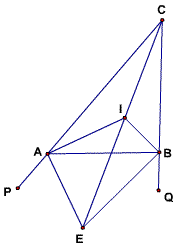
\includegraphics[scale=0.6]{xyz4Rr}
\end{center}
% https://s3.amazonaws.com/classroom.artofproblemsolving.com/Classes/GeomOlympiad/Images/xyz4Rr.gif


(In the below, $a$, $b$, $c$ are the usual $a = BC$, $b = AC$, $c = AB$)


    \begin{enumerate}
        \item Show that $AIC \sim EBC$ and $BIC \sim EAC$.
        
        
        \item Prove$$[EACB] = \dfrac{bxy}{2z} + \dfrac {br}2 + \dfrac {a^2br}{2z^2} = \dfrac{ axy}{2z} + \dfrac {ar}2 + \dfrac {b^2ar}{2z^2}$$
        
        
        \item Show that:$$ab - z^2 = \dfrac {xyz}r.$$
        
        
        \item Prove that:$$ \dfrac {ab - z^2}2 \cdot \sin C = rc. $$
    \end{enumerate}
\end{sketch}

\begin{mdsoln}
    \ \\
    \textbf{Solution 1} outline (the solution suggested by the hints, but much longer than the other solutions below!):
Extend $CI$ to the point $E$ such that $AE$ and $BE$ are exterior angle bisectors of $ABC$. Set $a = BC$, $b = CA$, $c = AB$.

Since $\angle EAI = 180^\circ - \angle IBE = 90^\circ$, $AEBI$ is cyclic, so
\[
\angle BEC = \angle BEI = \angle BAI = \angle IAC
\]Since we also have $\angle ECB = \angle ACI$, we can conclude that $\triangle BEC\sim \triangle IAC$. Likewise, $\triangle AEC\sim \triangle IBC$.

From $\triangle BEC\sim \triangle IAC$, we get
\[
[BEC] = [IAC]\left(\frac {BC}{IC}\right)^2 = \frac {1}{2}br\left(\frac {a}{z}\right)^2 = \frac {a^2br}{2z^2}
\]From $\triangle AEC\sim \triangle IBC$, we get
\[
AE = \frac {IB\cdot AC}{IC} = \frac {yb}{z}
\]Hence, the area of right triangle $IAE$ is
\[
\frac {1}{2}IA\cdot AE = \frac {bxy}{2z}
\]Therefore,
\[
[AEBC] = [IAE] + [IAC] + [BEC] = \frac {bxy}{2z} + \frac {br}{2} + \frac {a^2br}{2z^2}
\]Likewise,
\[
[AEBC] = \frac {axy}{2z} + \frac {ar}{2} + \frac {b^2ar}{2z^2}
\]Subtracting these two expressions yields
\[
0 = \frac {(b - a)xy}{2z} + \frac {(b - a)r}{2} - \frac {(b - a)abr}{2z^2}
\]Multiplying by $\frac {2z^2}{r(b - a)}$ gives us
\begin{eqnarray}0 & = & \frac {xyz}{r} + z^2 - ab\end{eqnarray}

\begin{lemma}
    $ab - z^2 = 2rc/\sin C$.
\end{lemma}
\begin{proof}
    Let $P,Q,R$ be the feet of the altitudes from $I$ to $BC,CA,AB$, respectively. Then, it is easy to see that $rc = [IQABP]$.
\end{proof} 

Now observe that
\begin{eqnarray*}\frac {z^2\sin C}{2} & = & z(z\cos (C/2))\sin C/2 \\
& = & (IC)(QC)\sin \angle QCI \\
& = & [IQCP]\end{eqnarray*}Hence,
\begin{eqnarray*}rc & = & [IQABP] \\
& = & [ABC] - [IQCP] \\
& = & \frac {ab\sin C}{2} - \frac {z^2\sin C}{2}\end{eqnarray*}from which the Lemma follows.
\vspace{6pt}

Now, substituting the expression from the Lemma into equation (1) yields
\[
0 = \frac {xyz}{r} - \frac {2rc}{\sin C}
\]implying that
\[
xyz = 2r^2\left(\frac {c}{\sin C}\right) = 2r^2(2R) = 4Rr^2
\]finally finishing the proof.

\vspace{10pt}
\textbf{Solution 2} outline (by Valentin Vornicu):
We can easily show using the Bisector Theorem that $AI = \dfrac {b + c}{a + b + c} w_a$, where $w_a$ is the length of the internal angle bisector from $A$. The relation becomes
\[
w_a w_b w_c (b + c)(c + a)(a + b) = 4Rr^2 \cdot 8s^3 .
\]But $rs = S$, so
\[
w_a w_b w_c (b + c)(c + a)(a + b) = 32 R S^2 s.
\]We also know that $4RS = abc$, and $w_a = \dfrac {2bc}{b + c} \cos \dfrac A2$, so
\[
8a^2b^2c^2 \cos \dfrac A2 \cos \dfrac B2 \cos \dfrac C2 = 8 abc Ss
\]so we only have to prove that
\[
abc \cos \dfrac A2 \cos \dfrac B2 \cos \dfrac C2 = Ss
\]But we know that $\cos \dfrac A2 = \sqrt {\dfrac {s(s - a)}{bc} }$, so the equality becomes
\[
\sqrt { s(s - a)(s - b)(s - c) } = S
\]which is as we all know the famous Heron's formula.

\vspace{10pt}

\textbf{Solution 3} outline:
Observe that the area of triangle $[BIC]$ is
\[
\frac {1}{2}yz\sin \angle BIC = \frac {1}{2}ar
\]Since $\angle BIC = 90^\circ + A/2$, this means that $\cos (A/2) = \frac {ar}{yz}$ so
\begin{align*}[ABC] & =  bc\sin(A/2)\cos(A/2) \\
& =  \frac {abcr\sin(A/2)}{yz}\end{align*}Then, $\frac {abc}{4R}  =  \frac {abcr\sin(A/2)}{yz}$, so
\[
4Rr^2 = \left(\frac {r}{\sin(A/2)}\right)yz = xyz
\]as desired.

\end{mdsoln}

